\documentclass{beamer}

% for themes, etc.
\mode<presentation>
{ \usetheme{metropolis} }
%{ \usetheme{boxes} }

\usepackage{times}  % fonts are up to you
\usepackage{graphicx}

% these will be used later in the title page
\title{CHPC WLCG Tier2 Facility and SA Grid Operations}
\author{Sean Murray \\
    ALICE \\
    CHPC \\
    CSIR 
}
\date{October 24 2017}

% note: do NOT include a \maketitle line; also note that this title
% material goes BEFORE the \begin{document}

% have this if you'd like a recurring outline
\AtBeginSection[]  % "Beamer, do the following at the start of every section"
{
\begin{frame}<beamer> 
\frametitle{Outline} % make a frame titled "Outline"
\tableofcontents[currentsection]  % show TOC and highlight current section
\end{frame}
}

\begin{document}

% this prints title, author etc. info from above
\begin{frame}
\titlepage
\end{frame}

\section{WLCG}

\begin{frame}
\frametitle{What is the WLCG}
\centering{
\includegraphics[scale=0.4]{WLCG-TiersJun14_v9.png}
}
\end{frame}
\begin{frame}
\frametitle{WLCG Map of Sites}
\centering{
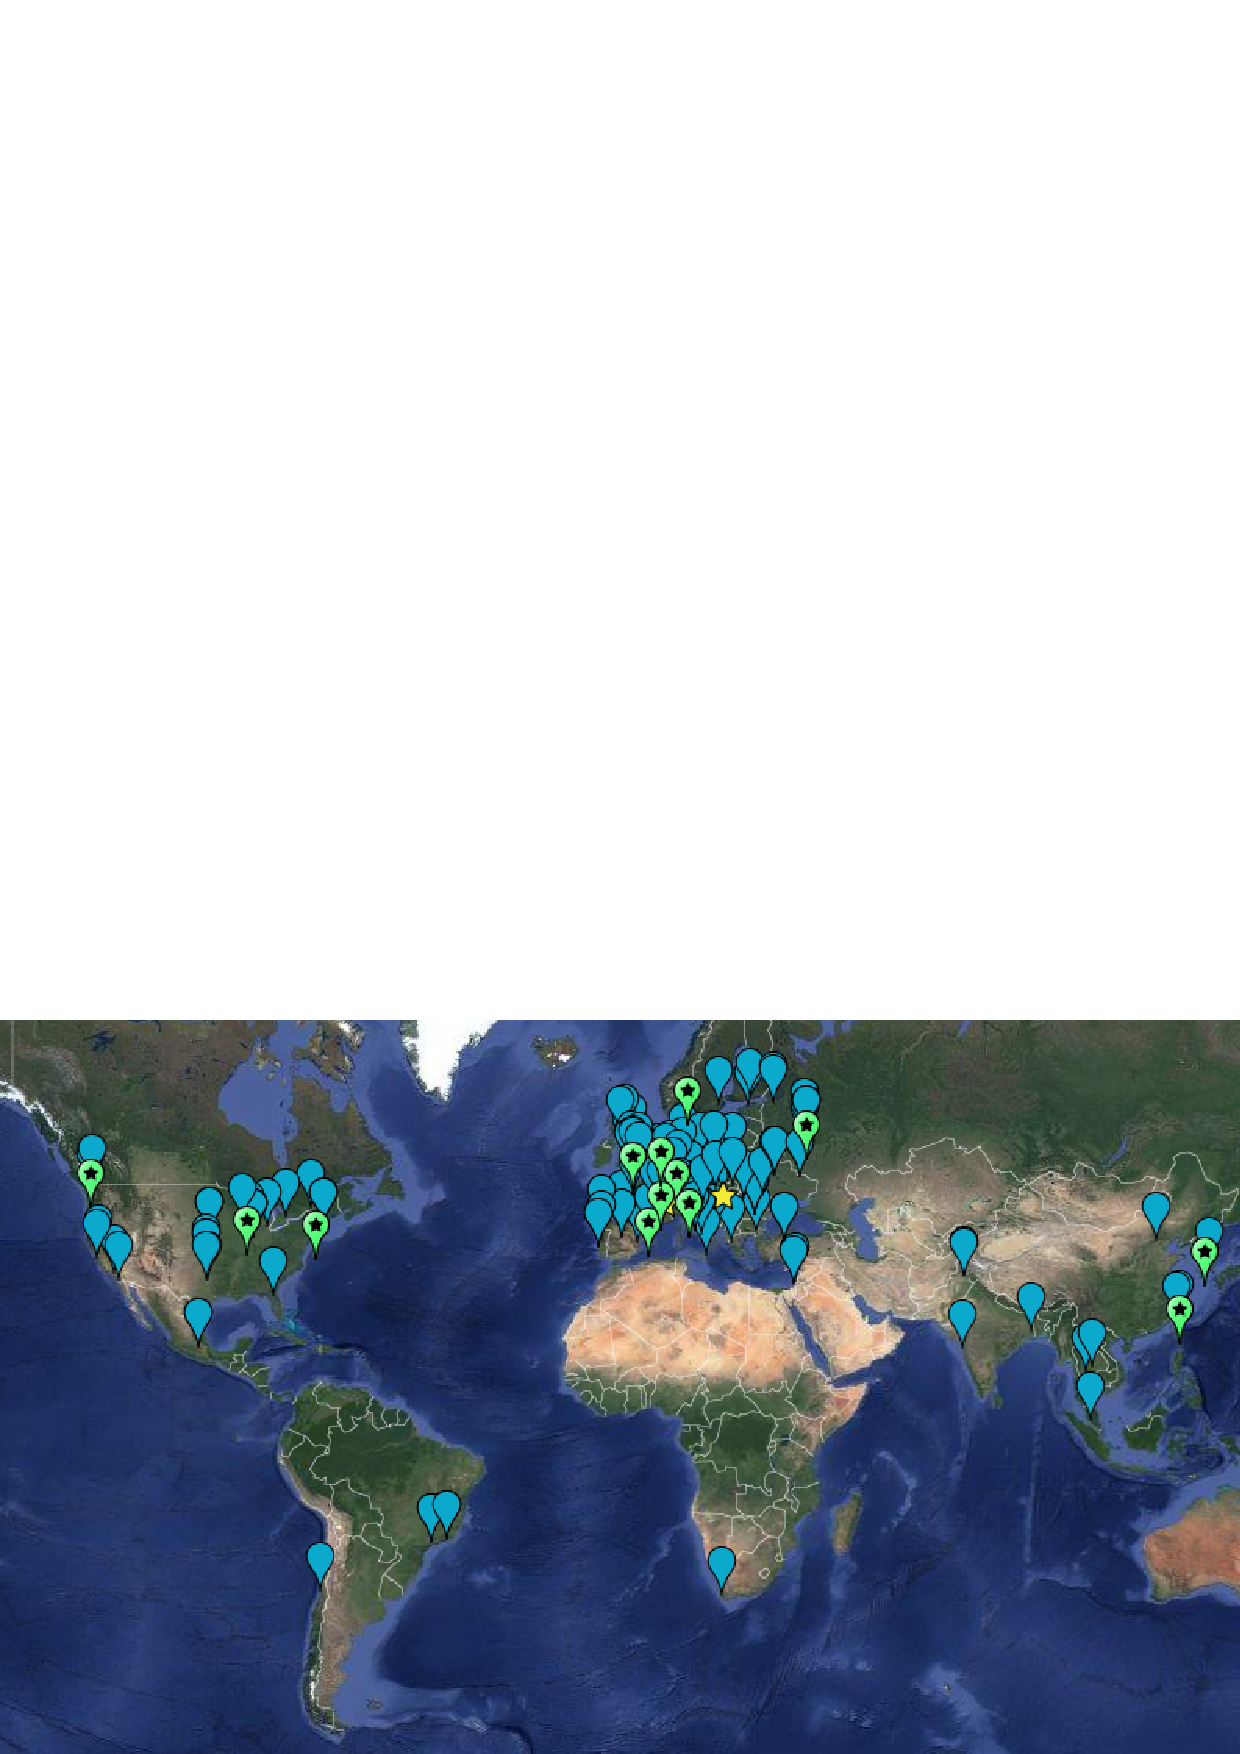
\includegraphics[scale=0.5]{WLCG-Sites.png}
}
\end{frame}

\begin{frame}
\frametitle{Commitments}
According to Tender :
\begin{itemize}
  \item ALICE 600 cores
  \item ATLAS 600 cores
  \item ALICE 400TB
  \item ATLAS 400TB
\end{itemize}
According to :
https://wlcg-rebus.cern.ch/apps/pledges/resources/
\begin{itemize}
    \item 6000 HEPSPEC06 cores (c. 560 of our cores) [2018=10k]
    \item 100TB storage [2018=1.5PB and 800TB]
  \item All ALICE.
  \item now equal ALICE and ATLAS (?)
  \item 212Mbps International Traffic.
\end{itemize}
\end{frame}

\begin{frame}
  \frametitle{Computing Infrastructure}
  \centering{
  \includegraphics[scale=0.30]{CHPCConnectivityDiagram.jpg}
  }
\end{frame}

\begin{frame}
  \frametitle{Current hardware}
  \begin{itemize}
    \item 50 nodes of 48 cores 192GB RAM and 2x800TB of SSD, 2 bonded 1G.
    \item 28 nodes of 48 cores 96GB RAM and 1TB SATA, QDR infiniband
    \item c.100TB of Lustre on the 28 nodes with QDR infiniband. --dead
    \item c. 1PB luster 4 IB FDR IB, -- dead migrating to beegfs/eos
    \item 9 management servers, lower spec
  \begin{itemize}
    \item compute element (head node,ce),
    \item storage element 2 redirectors, 2 storage nodes with direct attached multipath storage
    \item authentication, user interface (gone), monitoring, provisioning, site bdii.
  \end{itemize} 
    \item 16 blades of MD1000e, 384 cores. \color{red}{\bf IB connection}
  \end{itemize}
\end{frame}

\begin{frame}
  \frametitle{Current Storage}
  \begin{itemize}
    \item 383TB EOS for ALICE, down from 440TB
    \item 252 TB EOS for ATLAS, down from 400TB
    \item 107 TB lustre for 34 nodes.
    \item 1001 TB lustre 4 management nodes, 6 OSTs
    \item Quotes coming for 2PB EOS.
    \item \color{red}{400TB ALICE}
    \item \color{red}{400TB ATLAS}
  \end{itemize}
Reduction in data sizes is due to reorganisation for reliability.
\end{frame}


\begin{frame}
\frametitle{Storage questions}
    \begin{itemize}
        \item c. 1PB hardware lock in ?
        \item c. 1PB eos/beegfs/lustre reinstall
        \item 2PB EOS configured how?
    \end{itemize}
\end{frame}


\begin{frame}
  \frametitle{Availability / Reliability}
  So who monitors us :
  \begin{itemize}
    \item WLCG
    \item EGI
    \item ALICE
    \item ATLAS
    \item Local via zabbix/grafana and racktables(replacing with foreman plugin)
  \end{itemize}
There are a lot of eyes, ignoring the ones in this room.\\
\vspace{0.5cm}
\centering{
\begin{tabular}{|c|r|r|r|r|}
    Function     &  July & August & September & Year \\ \hline 
    Availability &  100   &  100     & 100 & 98.6 \\ \hline
    Reliability  &  100    &  100    & 100 & 99.5 \\ \hline
\end{tabular}

}
\vspace{0.5cm}
\end{frame}

\begin{frame}
  \frametitle{Grafana ALICE}
  \centering{
  \includegraphics[scale=0.2]{ALICEStatus.pdf}
  }\\
  This is currently being expanded to pull in more from MonaLisa, and more experiment and storage specific
  metrics to help to trivialy diagnose and forewarn problems. We want to know before everyone else.\\
    How else are we to hide our errors ....
\end{frame}

\begin{frame}
  \frametitle{Grafana ALICE}
  \centering{
  \includegraphics[scale=0.2]{Tier2Bandwidth.pdf}
  }\\
\end{frame}

\begin{frame}
  \frametitle{Tier2 Processing}
  \begin{itemize}
      \item ATLAS processing, pilot jobs start and then get work packages, data from Italy(T1).
    \item ALICE processing, job agents and leave it to central services, vobox.
    \item ops jobs fail due to starvation from alice. currently a dedicated machine, batch upgrade to fix.
    \item all software is distributed via cvmfs, both experiments.
    \item Both experiments have something similar to code-rade, an entire ecosystem of modules, versions, builds, etc.
    \item still no official validation on CC7.
  \end{itemize}
\end{frame}

\begin{frame}
  \frametitle{Tier2 Storage operations}
  Thankfully both experiments use xrootd. ATLAS will soon deprecate SRM.
  \begin{itemize}
    \item ALICE has its own authentication system, controlled centrally from CERN.
    \item ALICE has one big block of storage.
    \item ATLAS uses grid pool accounts, more standard grid.
    \item ATLAS has various storage's on site, cut up locally.
    \item ATLAS on puppet, ALICE will go on puppet when upgraded, upgrade in eos required for ipv6(xrootd4).
  \end{itemize}
\end{frame}


\begin{frame}
  \frametitle{Devops}
    \begin{itemize}
            \item I am a software engineer and writing software is what I enjoy, preferably computational physics and hardware stuff.
                \item So in the well trodden path of a theoretical physicist.
                    \item Think of a cow as a sphere .....
                        \item Lets approximate sys admin as a software problem.
                        \item I want everything in git and tested, and those tests automated.
    \end{itemize}

\end{frame}
\begin{frame}
  \frametitle{Philosophy}
  \begin{itemize}
    \item Keep It Simple Simpleton.
    \item Only use nonproprietary software.
    \item Stand on whom evers shoulders/heads/toes/knees I can. (Leverage the tools available)
    \item Abstract sys admin to a Software Engineering problem.
    \item Let me get back to the things that I enjoy ALICE O2, computational physics, machine learning etc.
  \end{itemize}
\end{frame}

\begin{frame}
  \frametitle{Simple Solution}
    \centering{Switch everything off for 4 or 5 months while we redo \bf{everything}, \color{red}{\bf BUT:}}
    \center\includegraphics[scale=0.5]{MOU-pic.pdf} \\
    \centering{Sadly we have an MOU to fullfill.}
\end{frame}

\begin{frame}
  \frametitle{the plan}
  \begin{itemize}
    \item Keep site up and processing maintaing our Tier 2 status.
    \item incrementally replace systems.
    \item We now have a MD1000e, on infiniband, a place to test configurations and deligate to batch
        we not playing.
  \end{itemize}
\end{frame}


\begin{frame}
  \frametitle{upgrades}
  \begin{itemize}
    \item attempts to delay till CC7 validation have failed.
    \item Puppify, to auto site deployment.
    \item Transition to foreman from xcat.
    \item Rewire whole network, re-power to monitored pdu, and monitor all.
    \item Add inherent redundancy into 10G interfaces on ce,se,se2.
    \item Reinstall while TRYING to keep A/R. problems are vobox and ce. 
    \item Storage, we now have approval for getting quotes, to fullfil our pledges for next year.
  \end{itemize}
\end{frame}
\begin{frame}
  \includegraphics[scale=0.25]{ALICEProcessing-Grafana.pdf}\\
  \includegraphics[scale=0.25]{ATLASProcessing-Grafana.pdf}\\
  \includegraphics[scale=0.25]{Server50-Grafana.pdf}\\
  \includegraphics[scale=0.25]{GrafanaMenu.pdf}
\end{frame}


\section{SAGrid, user analysis}
\begin{frame}
\frametitle{28 nodes}
28 of the 34 nodes came back for SAGrid and HEP when idle.
\begin{itemize}
  \item Go back to SAGrid to support anybody on SAGrid VO.
  \item HEP user analysis, based on federated identities, no user account admin.
  \item either HEP user supplies their own eco system with job or build their custom ecosystem via code-rade.
  \item code based on CODE-RADE, or LHC experiments.
  \item O2 dev for O2 development with dds/mesos/pbs. (no gpu/fpga)
  \item \color{red}{Local Storage for users, eos and lustre.}
\end{itemize}
\end{frame}

\begin{frame}
  \frametitle{deployment/provisioning}
  Foreman \ldots
  \begin{enumerate}
    \item deployment
    \item configuration, puppet, chef, salt, ansible.
    \item monitoring.
  \end{enumerate}
  Not using the fully integrated puppet/foreman as i prefer to be 
  tool agnostic, or at least strive for it. This might change.
\end{frame}


\begin{frame}
  \frametitle{puppet}
  A method/system to maintain a system in a known state.\\
  hiera, a key value store used by puppet.\\
  We store all site specific information in hiera, tightly integrated into puppet..
\end{frame}

\begin{frame}
\frametitle{AAROC Devops and r10k}
\begin{itemize}
  \item r10k branches are mapped to environments (dev, testing, production). Option to replace with foreman
  \item Cant be under AAROC, so chpctier2, production branch will be synced to aaroc/devops/chpc.
  \item 3 branches, dev, testing and production, currently only use production.
  \item all puppet except for eos is standard from other places, yaim is a pain.
      \item is mostly the R10k file and hiera for site specific information.
\end{itemize}
\end{frame}

\begin{frame}
  \frametitle{Testing}
  Devops requires some form of automated testing.
  \begin{itemize}
    \item Unit testing via rspec.
    \item Function testing.
    \item Fact testing.
    \item System testing.
  \end{itemize}
\end{frame}

%explain beaker testing. give example
\begin{frame}
    \frametitle{Beaker}
    \begin{itemize}
        \item Getting there .... \\
        \item Foreman templates written for some of beaker.
        \item Trying to integrate beaker tests and zabbix tests so tests are the same live and simulated. (pet project)
    \end{itemize}
    \end{frame}
\begin{frame}
    \frametitle{Beaker Pretty interface}
    Not surprisingly we get to a software engineering test case website ...\\
    \includegraphics[scale=0.25]{BeakerTest.pdf}
\end{frame}

\begin{frame}
    \frametitle{Beaker Pretty interface}
    \includegraphics[scale=0.25]{BeakerDetail.pdf}
\end{frame}

\begin{frame}
    \frametitle{Where to test}
    This is currently done on my desktop .....\\
    But not a standard dekstop
    \center {\bf BUT }
    \includegraphics[scale=0.25]{M1000e.pdf}
\end{frame}
\begin{frame}
  \frametitle{Monitoring}
  \begin{itemize}
    \item zabbix all data ends up here.
    \item grafana on zabbix.
    \item racktables with zabbix link, foreman plugin seems to do an easier job for our purposes.
    \item foreman
    \item monalisa
    \item have singular sources of authority. idrac mostly.
    \item all zabbix templates, items etc. on github, not really devops, and deployed by node type.
  \end{itemize}
\end{frame}

\begin{frame}
    \frametitle{TheForeman}
    \begin{itemize}
            \item Deploy and maintain the entire lifecycle of a machine.
            \item Deploy to cloud (numerous),
            \item deploy containers.
            \item monitor health e.g. puppet status.
            \item Combined with Katello and pulp, maintain package configurations (ignored)
            \item <2->Why ditch so much functionality? 
            \item <3->puppet-yum gets us back to {\color{red} {\bf everything}} in a series of git repos. Remember where I am coming from.
            \item <4->Replace r10k (at least how we use it) and keep the different branches of puppet for dev/test/prod.
    \end{itemize}
    We currently use it as almost a cobbler replacement, this might change.
\end{frame}

\begin{frame}
  \frametitle{network}
    This is \color{red}{critically} important for us.   
    \begin{itemize}
            \item All public interfaces are 1G cables across server room.
                \item change to dual 10G connections to switch.
                    \item 10G fibre to SANREN.
                        \item Shallow buffered swith, but in HA config.
    \end{itemize}
\end{frame}

% TODO insert pic of bandwidth from monalisa.
\begin{frame}
    \frametitle{Testing}
    We have been through a bout of testing, now moving to own network so can test further.
    \begin{itemize}
            \item Move outside CHPC network.
    \item Dedicated 10G to SANREN.
    \item PerfSonar installed.
        \item Test cleanly on our minimally buffered 10G Force10 Switch. Anybody want to loan us a 10G deep buffered switch to test.
    \end{itemize}
    \end{frame}

\begin{frame}
    \frametitle{Testing}
    \includegraphics[scale=0.35]{BandwidthTests.pdf}
\end{frame}

\begin{frame}
    \frametitle{Flies in the ointment}
    \begin{itemize}
            \item <1->Just when you think you on top of it .....
                \item <2-> Can not run tests on git update, waaaay to slow, but that is the least of the problems.
                    \item <3-> ALICE Job agents run for 28 hours
                        \item <4-> ATLAS pilot jobs run for c. 48 hours.
                            \item <5-> Any real test would take c. 72 hours to test properly with out annoying people.
                                \item <6-> We could just not care ....
                                    \item <7-> But we want real tests, it helps you sleep at night.
    \end{itemize}
\end{frame}



\begin{frame}
  \frametitle{bandwidth - Does ANYBODY ever have enough.}
  We were graciously donated a 1Gbps test.\\
  We used it all.\\
  We need more\ldots\ldots\ldots \\
  We have cables on order and then will upgrade to 10Gbps for testing purposes.
\end{frame}
\begin{frame}
    \frametitle{bandwidth yesterday}
\center    \includegraphics[scale=0.25]{Tier2Bandwidthcrop.pdf} \\ % TODO scale the crop the image.
Note the blue part, as our storage gets used the blue, international storage transfers becomes more significant than the rest. This
will become even worse once we get our 2PB installed (and used).
\end{frame}
\begin{frame}
  \frametitle{Summary}
  \begin{itemize}
    \item<2-> remove as much human contact as possible.
    \item<3-> abstract as much away to bot and psuedo bots
    \item<4-> let the science take priority.
    \item<5> William and I can sit back, drink espresso and watch some graphs ....
    \item<6> FROM THE BEACH !
  \end{itemize}
\end{frame}

\section{Backup Slides}

\begin{frame}
  \frametitle{LHCOPN}
  \centering{
  \includegraphics[scale=0.4]{map-lhcopn.png}
  }
\end{frame}

\begin{frame}
  \frametitle{IOU table}
  \includegraphics[scale=0.51,trim={1cm 5cm 1cm 18cm},clip]{mou_page23.pdf}\\
  \includegraphics[scale=0.51, trim={1cm 10cm 1cm 2cm},clip]{mou_page24.pdf}
\end{frame}

\begin{frame}
  \frametitle{mou table}
  \includegraphics[scale=0.5, trim={1cm 7cm 1cm 11cm},clip]{mou_page25.pdf}
\end{frame}

\end{document}
